\documentclass{article}

\usepackage{float}
%\usepackage{sidecap}
%\usepackage{csquotes} % ещё одна штука для цитат
\newtheorem{theorem}{Определение} % чтобы заработало окружение теорем


%Для мобилок
%\usepackage[left=20mm,right=20mm,top=20mm,bottom=20mm, paperwidth=150mm, paperheight=200mm]{geometry}




\usepackage[T2A]{fontenc}
\usepackage[utf8]{inputenc}
\usepackage[russian]{babel}

\usepackage{amsmath}

\usepackage{graphicx}

\usepackage{wasysym}
\begin{document}
 
\tableofcontents
 
\section{Механика}


\subsection{Кинематика}
\subsubsection{Введение}
\begin{theorem}
Основное понятие механики - движение, т.е. перемещение тела по отношению к другим телам. Без этих тел говорить о движении нельзя - оно относительно

\copyright{Ландау}
\end{theorem}


\begin{theorem}
Механика - раздел физики, в котором изучается простейшая форма движения материи - механическая, т.е. движение в пространстве и времени. Измерение расстояний осуществляется линейкой, времени - часами.

\copyright{Иродов и Савельев}
\end{theorem}

\begin{theorem}
Часы связаны с периодическими процессами, идущими с высокой степенью точности и повторяемостью, например колебания маятника или часового механизма

\copyright{Крымский, Кериченко}
\end{theorem}



Родоначальник классической механики - механики малых скоростей и абсолютного времени - \textbf{Ньютон}. Также серьезный вклад в классическую физику внес \textbf{Галилео Галилей}. Родноачальник релятивистской механики - физики больших скоростей и относительного времени - \textbf{Эйнштейн}

Согласно \textbf{СТО}, пространство и время неразрывно связаны, образуя четырехмерное \textbf{пространство-время}. Из \textbf{ОТО} следует, чтопространство гравитирующих масс искривляет пространство и влияет на ход времени.Еще одним ограничеснием на \textbf{Ньютоновскую механику} является \textbf{Квантовая механика}. Её родоначальники: \textbf{Н. Бор, Э. Шредингер, В. Гейзенберг, П. Дирак, В. Паули}.

Если поправки Эйнштейна важны на больших скоростях (близких к скорости света), то поправки, вносимые квантовой механикой, начинают наиболее ярко проявляться при изучении атомов и элементарных частиц. Тем не менее, \textbf{Классическая Ньютонова механика} продолжает быть справедливой для объектов макромира, скорость которых значительно ниже скорости света.

\subsubsection{Системы отсчета.Закон инерции Галилея(Первый закон ньютона).Инерциальные системы отсчета.}
\begin{theorem}
Совокупность тел, которые условно считаются неподвижными и относительно которых рассматривается движение других тел, называется системой отсчета.

\copyright{Ландау}
\end{theorem}


\begin{theorem}
Система отсчета - произвольным образом выбраноое тело или стстемы тел, относительно которого(ых) определяется положение всех прочих точек в простанстве. 

\copyright{Крымский, Кериченко}
\end{theorem} 

Если С.О. совпадает с самим телом, то тело будет \textbf{покоиться},  а в других с.о. - двигаться,причем в каждой с.о. - по-разному, т.е. по разным траекториям. В этом определении появляется очень важный термин \textbf{траектория}

Если тело находится настолько далеко от других тел,что не испытывает с их стороны никакого воздействия, то говорят, что это тело \textbf{свободно двигается}. 

\begin{theorem}
Если в качестве С.О. выбрать систему, связанную со свободно  двигающися телом, то в такой С.О. свободное движение других тел происходит \textbf{равноускоренно} и \textbf{прямолинейно}, т.е. описывается постояннй скоростью($v=const$). Такие С.О. называют инерциальными, сокращенно - ИСО. Это утверждение носит название \textbf{Закона инерции Галилея aka Первого Закона Ньютона}.
\end{theorem}



\begin{theorem}[Школьная формулировка Первого Закона Ньютона]
Если в некоторой СО сила, действующая на тело $\vec{F}=0$, то тело в этой СО движется прямолинейно и равномерно, а сама СО называется \textbf{инерциальной}
\end{theorem}

\begin{theorem}[Ещё одна формулировка Первого Закона Ньютона]
\textbf{Инерциальные системы отсчета} существуют, причем их бесконечное количество. Если некоторая система движется равномерно($\vec{v}=const$) относительно ИСО, то эта система тоже является ИСО.
\end{theorem}

\begin{theorem}[Принцип эквивалентности]
\textbf{Классическая механика} Ньютона и \textbf{Специальная теория относительности} Эйнштейна основаны на постулате о отм, что все физическия явления протекают одинаково в любой ИСО. Другими словами, все ИСО \textbf{физически эквивалентны}, то есть \textbf{все законы природы имеют одинаковый вид} во всех ИСО. 
\end{theorem}

\subsubsection{Кинематика. Материальная точка. Радиус-вектоор. Декартовы координаты. Скорость}
 
\begin{theorem}
Кинематика - раздел механики, где рассматривается геометрическое описание движения тел, независимо от причин, обуславливающих это движение.\footnote{Причины движения - силы, см. лекцию 3}

 \copyright{Крымский, Кериченко}
\end{theorem}


\begin{theorem}
Материальная точка(МТ) - это объект, формой и размером которого в условиях задачи можно пренебречь. МТ - основной объект механики.
\end{theorem}

Рассмотрим движение \emph{Земли} вокруг \emph{Солнца}. \emph{Землю} \textbf{ в этой задаче} можно считать МТ. Но при изучении \emph{суточного вращения Земли} вокруг своей оси, считать ее МТ уже нельзя!

\paragraph{Декартовы координаты}
\begin{theorem}
Положение МТ в пространстве полностью определяестя заданием трех координат: декартовых $(x,y,z)$, полярных $(r, \phi, \theta)$, или циллиндрических $(r,\rho, \phi)$.

\copyright{Ландау}
\end{theorem}

\paragraph{Перевод систем друг в друга}\footnote{$r$ на чертеже - это $\rho$}

\begin{figure}[H]
\centering
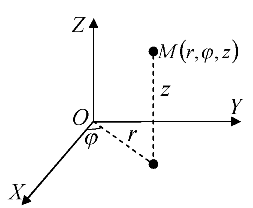
\includegraphics[scale=3.00]{coordinates.png}
\caption{}
\label{}
\end{figure}

$$
\text{Перевод полянрых координат}:
\begin{cases}
x = r \sin(\theta) \cos(\phi) 
\\
y = r \sin(\theta) \sin(\phi)
\\
z = r \cos(\phi)
\end{cases}
$$

$$
\theta - \text{Полярный угол;} \theta \in [0;\pi]
$$
$$
\phi - \text{Азимутальный угол;} \phi \in [0; 2\pi] 
$$

$$
\text{Перевод полянрых координат}:
\begin{cases}
x = \rho \cos(\phi) 
\\
y = \rho \sin(\phi)
\\
r^2 = \rho^2 + z^2
\end{cases}
$$

$$
\text{В Декартовых координатах}:
\begin{cases}
\vec{r} = x\vec{e_x} + y\vec{e_y} + z\vec{e_z} = \\
=\displaystyle \sum_{\alpha = 1}^{3} x_\alpha e_\alpha = x_\alpha e_\alpha (\alpha =1..3)
\\
e_i - \text{единичные векторы}
\\
x_i - \text{Координаты по разным осям}
\\
r^2 = x^2 + y^2 + z^2 = \rho^2 + x^2
\\
\rho^2 = x^2 + y^2 
\\
(e_{\alpha}x_{\alpha})^2=1
\\
e_x*e_y = e_x*e_z = e_y*e_z = 0
\\
\end{cases}
$$

Последнеее утверждение в переводе на человеческий означает, что все три $e_i$ взаимно препендикулярны
\begin{theorem}
совокупность трех величин $(x,y,z)$ образует \textbf{радиус-вектор} $\vec{r}$ частицы, направленный из точки $O$ - начала координат в точку $A$ - позицию частицы. 
\end{theorem}

\subsubsection{Траектория. Перемещение и путь материальной точки}
\begin{theorem}
Положение точки $A$  в пространстве в данный момент времени полностью определяется заданием зависимости $\vec{r}(t)$. С течением времени положение $A$ меняется(см. чертеж), так, что конец $\vec{r}$ описывает в пространстве некоторую кривую, называемую траекторией материальной точки $A$.
\copyright{Ландау}
\end{theorem}

\begin{figure}[H]
\centering
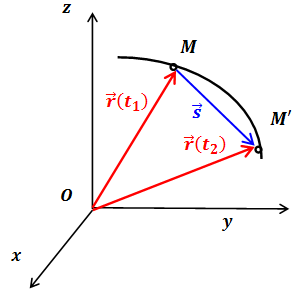
\includegraphics[scale=1.00]{trajectory.png}
\caption{}
\label{}
\end{figure}
Траектория м.быть окружностью радиуса $R$, параболой, прямой и т.д.
 
О материальной точке мы часто будем говорит также как о \textbf{частице}. В связи с тем, что М.Т. описывается тремя декартовыми координатами $(x,y,z)$, о ней часто говорят, что М.Т. обладает \textbf{тремя степенями свободы}.

\subsubsection{Скорость}
\begin{theorem}
Движение М.Т. характеризуется ее \textbf{скоростью}, при равномерном и прямолинейном движении значение скорости определяется просто как путь, проходимый частицей в единицу времени: $v=\frac{\Delta s}{\Delta{t}}$. 

В общем случае же, когда движение \textbf{неравномерно}, и меняет свое направление, скорость частицы определяется как \textbf{вектор}, равные частному от деления вектора \textbf{бесконечно малого} перемещения частицы $dS$ на соответствующий интервал времени$dt$:$\vec{v} = \frac{d\vec{S}}{dt}$.

 Направление $\vec{v}$ совпадает с направлением $\vec{dS}$, то есть в каждый момент времени скорость направлена \textbf{по касательной к траектории частицы}, в сторону движения.
\end{theorem}	

На рисунке изображена траектория движения некоторой М.Т., и отмечены ее радиус-векторы $\vec{r}$ и $\vec{r} + \vec{dr}$ в моменты времени $t$ и $t+dt$. Пользуясь правилом сложения векторов, легко убедиться, что \textbf{бесконечно малое смещение} точки $A$ равно разности радиус-векторов частицы в начальный и конечный моменты времени, то есть $d\vec{S}=d\vec{r}$. То есть скорость можно определить как $\vec{v} = \frac{d\vec{S}}{dt} = \frac{d\vec{r}}{dt}$. То есть скорость есть производная радиус-вектора частицы по времени.

Поскольку компонентами радиус-вектора $\vec{r}$ являются декартовы координат , то проекции скорости на оси координат $x,y,z$ равны производным: 
$$\vec{v_x} = \frac{d\vec{x}}{dt}$$
$$\vec{v_x} = \frac{d\vec{y}}{dt}$$
$$\vec{v_x} = \frac{d\vec{z}}{dt}$$
$$ \vec{r} = x\vec{e_x} + y\vec{e_y} + z\vec{e_z}$$
где $\vec{e_x}, \vec{e_y}, \vec{e_z}$ - три взаимно перпендикулярных единичных вектора.

Скорость наряду с положением является основной величиной, характеризующей состояние \textbf{движения } М.Т. Сотсояние частицы определяется, следовательно, шестью величинами: тремя координатами и тремя проекциями скорости.

\subsubsection{Закон сложения скоростей}

Установим связь между значениями скоростей $\vec{v}$ и $\vec{v}'$ Одной и той же М.Т. в двух разных системах отсчета $K$ и $K'$. Если за время $dt$ материальная точка переместилась относительно системы отсчета $K$ на величину $d\vec{s}$, а система $K$ переместилась в свою очередь относительно системы $K'$ на величину $d\vec{S}$, то из правила сложения векторов следует, что смещение М.Т. онсоительно системы $K'$ будет равно 

$$d\vec{S'} = d\vec{s} + d\vec{s}$$ 

Разделив обе части на интервал времени $dt$ и обозначив скорость $K$ относительно $K'$ через $\vec{V}$, получим \textbf{Правило сложения скоростей}:
$$\vec{v}' = \vec{v} + \vec{V}$$

Даже если скорости непостоянны, в любой момент времени

$$\vec{v}'(t) = \vec{v}(t) + \vec{V}(t)$$

Эта формула, связывающая скорости одной и той же М.Т. в разных системах отсчета - правило сложения скоростей.

\subsubsection{Абсолютность времени в Ньютоновской механике}

На первый взгляд правило сложения скоростей представляется совершенно очевидным. Необходимо, однако, иметь в виду, что оно основано на \emph{молчаливо} сделанном предположении об \textbf{абсолютном течении времени}. Мы считаем, что интервал времени $dt$, за который частица смещается на величину $d\vec{s}$ в системе $K$ равен интервалу времени $dt'$, за который частица смещается на величину $d\vec{S}'$ в системе $K'$.

Это предположение в действительности строго говоря неправильно. Время - тоже относительно, в СТО Эйнштейна, но следствия, вытекающие из неабсолютности времени, начинают проявляться только на скоростях, сравнимых со скоростью света $\vec{c} = 3*10^{10} cm/s$. Мы в дальнейшем в этом модуле будем рассматривать лишь 	$\vec{v}<<\vec{c}$, когда предположение об \textbf{абсолютности времени} хорошо оправдывается. 

Механика, основаная на предположении об абсолютности времени называется ньютоновской или классической. Только эту механику мы будем изучать в первом модуле. Основные ее законы были сформулированы Ньютоном в его трактате "Математические начала натуральной философии".

\subsubsection{Ускорение. Движение по окружности}
\paragraph{Ускорение}
В общем случае движения М.Т., ее скорость нерпрервыно меняется как по величине, так и по времени. Пусть за время $dt$ скорость изменилась на $d\vec{v}$. Если разделить их друг на друга, получим вектор ускорения $\vec{a} = \frac{d\vec{v}}{dt}$. Ускорение определяет изменение скорости частицы и равно производной от скорости по времени.

Если направление скорости не изменяеся, то есть М.Т. движется по прямой, то ускорение, очевидно, направлено по той же прямой и равно.

Кроме того, $\vec{a} = \frac{d^2\vec{S}}{d^2t}$

Легко также определить ускорение, если скорость меняется тоько по направлению, оставаясь постоянной по величине. Этот случай имеет место при прямолинейном равномерном движении М.Т. по окружности

\subsubsection{Центростремительное ускорение} $a_c = \frac{v^2}{R}$.

Пусть в некоторый момент времени скорость равна $\vec{v}$(см. рис. 1). Отложим его от некоторой точки C(рис. 2). При равномерном движении по окружности конец $\vec{v}$(точка А на рис. 2) также равномерно движется по окружности радиуса $|\vec{v}|$ равного абсолютному значению скорости. Ясно, что скорсоть перемещения точки $A$ на рисунке 2 будет ускорение исходной частицы $P$ на рисунке 1, так как перемещение точки $A$ за время $dt$ равно $d\vec{t}$ и следовательно скорость точки $A$ на рисунке 2 равна $\frac{d\vec{v}}{dt} = \vec{a}$. Эта скорость имея направление касательной к окружности, с центром $C$ на рис. 2, препендикулярна вектору $\vec{v}$. На рисунке он аобозначена $\vec{a}$

Если скорость $\vec{v}$ перпендикулярна $\vec{a}$ на \textbf{вспомогательном рисунке}, то v должна быть перпендикулярна a и на основном рисунке. Таким образом, ускорение М.Т., равномерно движущейся по окружности, перпендикулярно скорости. Определим величину \textbf{центростремительного ускорения} $\vec{a}$. За время полного обращения точки $P$ по окружности с центром в точке $O$, точка $A$ на вспомогательном рисунке пробежит \textbf{всю окружность с центром в точке $C$}, то есть пройдет путь $\vec{S} = 2 \pi \vec{v}$. Обозначим период обращения точки $P$ вокруг $O$ и точки $A$ вокруг $C$ как $T$.


Среднее по времени:

$$<f>_t = \frac{1}{T} * \int^T_0f(t)dt$$

Тогда на вспомогательном рисунке $2 \pi \vec{v} = \vec{a}t$, то есть путь равен произведению скорости движения $A$, то есть фактически модуля ускорения $|\vec{a}|$ на время движения $T$. Тогда 
$$\vec{a} = \frac{2\pi v}{T}$$

Аналогично на основном рисунке $$T=\frac{2 \pi r}{v}$$

Подставив одно выражение в другое, получим следующее:

$$
\begin{cases}
\vec{a} = \frac{2\pi v}{T}
\\
T=\frac{2 \pi r}{v}
\end{cases}\Rightarrow a = \frac{v^2}{r}
$$

Центростремительное ускорение равно квадрату скорости, деленному на радиус окружности

Итак, если скорость меняестя только по величине, то направление ускорения совпадает с направлением корости(для движения по прямой). Если же скорость меняется тольеко по направлению(движение по окружности), то векторы скорсоти и ускорения взаимно перпендикулярны.

В общем случае, когда скорость $\vec{v}(t)$ меняется как по величине, так и по направлению, ускорение имеет \textbf{ две компоненты}: одну - \emph{тангенциальную(касательную)}, вдоль скорост $\vec{v}$ и другую -\emph{нормальную}, перпендикулярную скорости $\vec{v}$. Полное ускорение равно их сумме: $$\vec{a} = \vec{a_n} + \vec{a_t}$$

Касательная составляющая ускорени равно производной от величины скорости $d\vec{v}$ по времени $d\vec{T}$

Нормальная составляющая равна $\frac{v^2}{r}$, где $r$ - радиус кривизны. Качественно, радиус кривизны равен радиусу окружности, наилучшим образом аппроксимирующей траеторию на данном малом участке траектории. Для движения по прямой радиус кривизны бесконечно велик. 

В общем случае, любой малый участок траектории можно положить на плоскость и ввести его описание через $y=f(x)$. 

Обратный радиус кривизны равен модуля второй производной этой функции.
$$\frac{1}{R} = |\frac{d^2y}{dx^2}|$$

В общем случае радиус кривизна определяется именно так, через вторую производную функции траектории.

\paragraph{Другой, более традиционный вывод центростремительного ускорения}
При движении по окружности длина бесконечно малого перемещения равна длинне бесконечно малой дуги окружности радиуса $r$:$$dS = r d\phi$$
где $d\phi$ - бесконечно малое приращение угла $\phi$ - азимутального угла. За период обращения полное изменение $\phi$: $$\Delta \phi = 2 \pi$$ Но по определению, абсолютное згачение скорости есть производная от бесконечно малого перемещения $dS$ по времени $dt$. При этом радиус окружности $r=const$. Тогда $$v=\frac{dS}{dt} = r\frac{d\phi}{dt}$$. Величина $\frac{d\phi}{dt} = \omega$, 	где $\omega$ - угловая скорость. Она определяестя отношением бесконечно малого изменения угла $\phi$ к бесконечно малому промежутку времени $dt$, за корорый произошло это изменение угла.

$$
\begin{cases}
v=\frac{2\pi r}{T}
\\
v=\frac{2\pi r }{t}
\end{cases} \Rightarrow \omega = \frac{2\pi}{T}
$$

Это соотношение очень важно для всех периодических и колебательных движений.

Выведем соотношение между центростремительным ускорением $a$ и угловой частотой вращения $\omega$

$$
\begin{cases}
a = \frac{2\pi r}{\omega}
\\
\omega = \frac{2 \pi}{T}
\\
v= \omega r
\end{cases} \Rightarrow a = \omega^2r
$$

Центростремительное ускорение пропорционально квадарату угловой скорости, умноженному на радиус окружности.

\subsubsection{Матрицы}

$\begin{matrix}
	i & j & k\\
	1 & 0 & 2\\
	2& 3 & 1\\
\end{matrix}$

$\begin{matrix}
	a_{11} & a_{12} \\
	a{21}& a_{22} \\
\end{matrix}$


Детерминант(определитель) мартрицы - произведение $-a_{12}*a_{21}+a_{11}*a_{22}$

Иначе можно поступить, умножив каждый элемент строки или столбца, на определитель матрицы, получаемой вычеркиванием столбца и строки этого элемента. Знак определяется как $-1^{coeffs sum}$ Детерминант матрицы 1*1 равен значению единственного элемента.

Детерминант матрицы 3*3 равен произведению каждого элемента строки или столбца на детерминант соотыветствующей матрицы 2*2 

Применение детерминантов - расчет векторного произведения:
$$
a = a_i*\vec{i} +  a_j*\vec{j} +  a_k*\vec{k}
$$$$
b = b_i*\vec{i} +  b_j*\vec{j} +  b_k*\vec{k}
$$$$
|\vec{c}|=|\vec{a}*\vec{b}| = \begin{vmatrix}
	i & j & k\\
	a_x & a_y & a_z\\
	b_x& b_y & b_z\\
\end{vmatrix}
$$

Ускорение состоит из двух компонент: нормального $a_n$ и тангенциального $a_t$

нормальное ускорение считатется так: $$a_n = \frac{v^2}{\rho}$$

$a_t = \frac{dv}{dt}$

\subsubsection{Кинематика твердого тела. Виды движения твердого тела.}
На лекции 2 мы познакомились с двумя \textbf{основными} видами движения: равномерным прямолинейным и вращательным, то етсь равномерным движением по окружности.

До сих пор мы изучали дижение тел, которые можно было рассматривать в данных условия как материальные точки. Теперь мы перейдем к описанию таких движений, при которых существенно \textbf{конечная протяженность} тела. При этом мы будем считать тела \textbf{твердыми}(в мезанике часто говорят абсолютно твердыми). Под твердым понимается тело, взаимное расположение частей которого остается неизменным во время движения. Такое тело выступает при движении как \emph{единое целое}. Простейшим движение твердого тела является движение, при котором тело перемещается \textbf{параллельно самому себе}. Такое движение называется\textbf{ поступательным}.
\subsubsection{ Поступательное движение твердого тела.}
\begin{theorem}
При поступательном движении твердого тела \emph{все его точки имеют равную скорость $\vec{v}$} и описыают траектории одинаковой формы, смещенные по отношению друг к другу.
\\ 
\copyright{Ландау}
\end{theorem}

\subsubsection{Вращательное движение}
Другим простейшим движение твердого тела является вращение тела ворруг оси. При вращении разлиные точки тела описаывают окружности, лежащие в плоскостях, перпендикулярных оси вращения.

При вращательном движении все точки твердого тела движутся по окружностям, центры которых лежат на одной и той же прямой - \textbf{оси вращения}. Если $r$ - расстояние от точки до оси вращения $oZ$, то скорость равна произведению угловой скорости на радиус.

$$\vec{v} = \omega \vec{r}$$
 В механие твердого тела скорость называется скоростью твердотельного вращения. Она пропорциональна угловой скорости вращения $\omega$  и расстоянию от точки твердого тела $P$ до оси вращения.

Если вращение твердого тела происходит равномерно($\omega=const$), то как мы показали в лекции 2, угловая скорость связана с периодом вращения по формулам:
$$T = \frac{2\pi}{\omega}$$
$$\omega = \frac{2\pi}{T}$$

Вращение зарактеризуется направлением оси вращения и величиной угловой скорости. Их можно объединить вместе, введя \emph{вектор угловой скорости} $\vec{\omega}$. Такой вектор имеет величину равную $\omega$ и коллинеарен оси вращения. Из двух направлений оси вращения вектору гловой скорости принято приписывать направление, определяемое \emph{правилом правого винта}, то есть то, при вращении \emph{ввинчивается винт с правой резьбой}.

\subsubsection{Произвольное движение твердого тела. Движение твердого тела, параллельное плоскости}

Рассмотренные нами простейшие виды движения твердого тела - поступательное движение и вращение особенно важны в механике, потому что \emph{любое движение твердого тела сводится к их комбинации}

Рассмотрим движение твердого тела, параллельное некоторой плоскости. Такое движение иногда называют \emph{плоским движением}

Рассмотрим два последовательных положения тела $A_1$ и $A_2$. Из положения $A_1$ в положение $A_2$ твердое тело можно переместить следующим образом, используя комбинацию поступательного и вращательного движений:

В начале \emph{параллельным переносом} пожно перевести тело(и отрезок $OO'$ в нем) из положения $A_1$ в положение $A'$. Это поступательное движение твердого тела. А затем поворотом на угол $\phi$ отностиельно нижней точки отрезка $O$ в конечное положение $A_2$. Это вращательное движение твердого тела. 

В то же время, можно и наоборот: переместить тело из положения $A_1$ в $A_2$, в начале сделав параллельный перенос тела в положение $A''$, и тоже повернуть вокруг верхней точки $O$ на тот же угол $\phi$

При этом угол поворота во вращательно движении \emph{обязательно одинаков}, хотя точки \emph{мгновенной оси поворота} $O$ и $O'$ - различны. В то же время, длина пути поступательного движения(длина перемещения отрезка $OO'$) вообще говоря разная. Рассмотренный пример показывает, что любое произвольное движение твердого тела можно представить в виде совокупности поступательного движения всего тела со скоростью $\vec{v}$ какой-то его точки и вращения вокруг оси, проходящей через эту точку. При том поступательная скорость $\vec{v}$ зависит от того, какая из точек тела выбрана в качестве \emph{основной}. Обычно, в качестве основной выбирается \emph{центр масс(центр тяжести тела)}. Поступательная скорость $\vec{v}$ есть скорость центра масс. Точку центра масс в механике также часто называют \emph{центром инерции} тела. 

Угловая же скорсоть $\vec{\omega}$ от выбора основной точки не зависит. При любом выборе основной точки угловая скорость будет иметь одинаковую величину и направление. Можно сказать, что скорость поступательного движения имеет \emph{относительный характер}, а угловая скорость вращения твердого тела - \emph{абсолютный характер}


Каждый их векторов скорсои задается тремя проекциями, так тчо для знания скоростивсех точек твердого тела надо задать 6 независимых величин. Поэтому говорят, сто твердое тело - \emph{механическая система с шестью степенями свободы}. При этом в общем случае скорость твердого тела записывается

$$\vec{V} = (v_x, v_y, v_x)$$
$$\vec{\omega} = (\omega_x, \omega_y, \omega_z)$$

При этом в общем случае скорость твердого тела записывается как
$$\vec{v} = \vec{V} + [\omega*r]$$
\subsubsection{Мгновенная ось вращения}
\paragraph{Качение по плоскости как пример плоского движения твердого тела}
Итак, как мы уже говорили, плоским движением называется такое движение, при котором все точки тела движутся в плоскостях, параллельных \emph{одной и той же неподвижной плоскости}. 

При этом линейная скорость любой точки тела $\vec{v_0}$ перпендикулярна вектору угловой скорости $\omega$.
Пример плоского движения дает качение циллиндра по плоскости. Имеет место слкдующее утверждение: при плоском движении твердого тела любое \emph{бесконечно малое} движение можно представить как \emph{чистое вращение} тела вокруг некоторой оси. Эта ось назывется \emph{мгновенной осью вращения}. Решим данную заадачу по учебнику Савельева. Итак, $$\vec{V} = \vec{v_0} + [\omega/r]$$, причем эти два слагаемые для полной скорости параллельны или антипараллельны друг другу. Главная фишка в том, что в нижней точке $O'$ скорость поступательного движения $\vec{v_0}$ и скорсоть вращения $[\omega *r]$ противоположны. В то же время в верхней точке $O''$ они складываются. В нижней точке касания суммарная скорость равна нулю, в точке $O$ скорость равна $v_0$, а в верхней - $2v_0$

Тогда поступательное и вращательное двмжение(каение колеса можно) представить как чистое вращение вокруг мгновеено оси, проходящей через нижнюю точку $O'$. Действительно, тогда в точке $O'$
$$V = [\omega*0] = 0$$
В точке $O$
$$V = [\omega*r] = v_0$$

В точке $O''$
$$V = [\omega*2r] = 2v_0$$

Замечание: при неплосо=ком движении элементарное перемещение тела можно пердставить как поворот вокруг мгновенной оси лишь в том случае, если векторы $\vec{v0}$ и $\vec{\omega}$ перпендикулярны. Если угол межлу ними отличен от 90 то движение тела в каждый момент времени будет наложением двух движений: вращения вокруг оси и потсупательного движени вдоль этой оси.
\subsection{Динамика}
\subsubsection{Основные законы ньютоновской динамики.  Третий зн. Закон сохранения импульса.Движение центра масс} 
\begin{theorem}[Первый закон ньютона]
Всякое тело сохраняет состояние покоя или равномерного прямолинейного движения, пока и поскольку оно не понуждается приложенными силами изменять это состояние
\copyright{Крымский}
\end{theorem}


\subsubsection{Масса материальной точки, импульс}

Импульс $\vec{p}$ материальной точки связан простым соотношением со скоростью М.Т. 
$$\vec{P} = m\vec{v}$$
Коэффициент $m$ - характерная для каждой М.Т. постоянная - ее масса. Как показывает опыт, в классической механике масса тела не зависит от скорости. $$m= const$$

Замечание1. Строго говоря, в определение импульса входит \emph{инертная(иннерционая)} масса $m_i$, а в закон всемирного тяготения Ньютона входит \emph{гравитационная} масса $m_g$, но существует принцип эквивалентности Ньютона-Эйнштейна между инертной и гравитационной массой. Согласно этому принципу, инертная и гравитационная массы равны.

Замечание 2. В физической системе СГС масса измеряется в граммах, в инженерной СИ - в килограммах

\subsubsection{Сила. Второй закон Ньютона}
Если М.Т. совершает сободное движение, то есть не взаимодействует с окружающими телами, то сохраняется ее импульс, если взаимодействует - то ее импульс меняется со временем. Мы можем, следовательно рассмартивать изменение импульса М.Т. как меру воздействия на нее со стороны окружающих тел. Чем больше это изменение за единицу времени,тем интенсивнее воздействие.

Как мы уже обсуждали на прошлой лекции, для определения \textbf{воздействия }на М.Т. со стороны окружающих тел естественно рассматривать производную вектора импульса этой М.Т. по времени. Эта производная называется \textbf{силой $\vec F$}:
$$\vec F = \frac{d\vec{P}}{dt}$$


Такое определение характеризует одну сторону взаимодействия, а именно степень \emph{"реагирования"} М.Т. на воздействия на нее со стороны окружающих тел. Но с другой стороны, изучая взаимодействие М.Т. с окружающими телами, можно связать \textbf{силу этого взаимодействия} с величинами, характеризующими состояние М.Т. и состояние окружающих тел. 

Силы взаимодействия между М.Т. в классической механике оказываются зависящими только от расположения М.Т. Иными словами, силы, действующие между частицами зависят только от рассояния между ними, но не от скоростей частиц(это не так в СТО).

Характер зависимости сил от расстояний между частицами может быть во многих случаях установлен исходя из изучения тех физических явлений, которые лежат в основе взаимодействий между М.Т. Например, для закона всемирного тяготения Ньютона, сила обратно пропорциональна квадрату расстояния между двумя точками с масссами $M_1$ и $M_2$.
$$\vec{F} = G\frac{M_1 M_2}{r^3}*\vec{r}$$
Используем две стороны определения силы и обозначим через $\vec F$ выражение для силы, действующей на расссматриваемую М.Т. в зависимости от ее координат(а также, в общем случае, от величин, характеризующих свойства и расположение окружающих тел, например массы окр. тел в механике или их заряды в электростатике). Мы можем тогда записать равенство двух выражений для силы - изменение импульса М.Т. в ед. времени $\frac{d\vec P}{dt}$ и силы.
4$$\frac{dP}{dt} = \vec F(x,y,z...)$$

Так как импульс $P$ в классической механике равен $m\vec v$, то есть произведению массы и скорости, то уравенение движения М.Т. можно записать в виде:
$$\frac {d\vec P} {dt} = m \frac{d\vec v}{dt} = \vec v$$
Но по определению $\frac{d\vec v}{dt} = \vec a$
\\
Тогда получаем "школьный" вид II Закона Ньютона:
$$\vec{F} = m \vec a$$
$$\vec a = \frac{\vec F}{m}$$

При выводе II Закона Ньютона мы считали, что масса не меняется со временем. Таким образом, сила $\vec F$, действующая на М.Т. равна произведению ее ускорения на ее массу.

Подчеркнем однако,что второй закон Ньютона приобретает конкретный смысл только после того, как установлен вид силы $\vec F$ как функции координат системы. В этом случае(если вид функции $\vec F(\vec r)$ известен, уравнение движения позволяет в принципе определить зависимость скорости $\vec v$ и координат $\vec r = (x,y,z)$ времени $t$, то есть найти траекторию ее движения. При этом, помимо вида функции $\vec F(\vec{r})$, то етсь законов взаимодействия частицы с окружающими телами, должны быть заданы, как говорят, \emph{начальные условия}: положение и скорость частицы в некоторый  момент времени, принимаемый в качестве исходного.

Поскольку уравнение движения можно переписать в виде 
$$\vec{a} = \frac{d\vec v}{dt} = \vec Fm$$
то бесконечно малое приращение скорости $dv$ частицы за каждый интервал времени $dt$ определяется по формуле $$d\vec v = \frac{\vec F} m$$.
\\
А еще
$$d\vec r =\vec v dt$$
Отсюда ясно,что задание начального положения и начальной скорости частицы вместе со вторым законом Ньютона действительно достаточно для полного определения ее траектории, то есть ее дальнейшего движения. Уравнение  движения является векторынм уравнением, поэтому его можно переписать в виде трех уравнений, связывающих проекции ускорения и силы на оси $Ox, Oy, Oz$:
$$\vec F_\alpha = m \frac{d \vec{v_\alpha}}{dt}$$

При свободном движении М.Т., когда она не взаимодействует с другими телами, скорость ее в ИСО остается неизменной - по первому З.Н. Напротив, если М.Т. взаимодействуют друг с другом, то их скорости \emph{меняются с течением времени}. Изменения скоростей взаимодействующих друг с другом частиц не является однако \emph{поностью независимыми}, а связаны между собой. Пусть наша системы состоит из $N$ М.Т. Предположим, что эти М.Т. взаимодействуют меду собой, но\emph{ не взаимодействуют с окружающими телами}. Тогда для такой совокупности М.Т. можно ввести понятие \textbf{замкнутой системы}. 

Под замкнутой системой будем понимать совокупность М.Т., взаимодействующих друг с другом и не взаимодействующих с окружающими телами. Для замкнутой системы существует ряд величин, связанных со скоростями, и не меняющихся с течением времени.

Эти сохраняющиеся величины играют особенно важную роль в механике. Это импульс, энергия и момент импульса. Их называют иногда интегралами движения.

Одна из этих величин - полный импульс системы $P_\Sigma$. Он представляет собой векторную сумму импульсов каждой из $N$ М.Т.

\subsubsection{Закон сохранения импульса}
Сумма векторов $\vec p_i$, распространенных на все частицы замкнутой системы преставляет собой полный импульс 
$$P_\Sigma = \sum_{i=1}^Np_i = \sum_{i=1}^Nm_iv_i$$
где индексы нумеруют отдельные М.Т. Эта величина не меняется с течением времени. $$\vec P_\Sigma = const \Rightarrow \frac{d\vec {P_\Sigma}}{dt} = 0$$
Итак, полный мипульс замкнутой системы сохраняется. Это - закон сохранения импульса.

Закон сохранения импульса распадается на три закона - по одному на ось.
$$\vec P_{\Sigma_\alpha} = const$$

\subsubsection{Третий закон Ньютона}

Из ЗСИ следует, что 
$$\sum_{i=1}^{N}{m_i\frac{d\vec{v_i}}{dt}} = 0$$

Через определение силы:

$$\sum_{i=1}^{N} \vec F_i = 0$$

Расмотрим систему из двух тел, обозначив силы соответственно $\vec {F_{12}}$ и $\vec{F_{12}}$. Из уравнени выше следует:

$$\vec{F_{12}} = - \vec{F_{21}}$$

Сила действия равна силе противодействия по модулю, но противоположны по направлению - в этом состоит \textbf{Третий Закон Ньютона}

\subsubsection{Центр инерции, центр масс}

С ЗСИ в классической механике связано важное свойство массы - закон сохранения массы. Чтобы понять содержание этого закона, для замкнутой системы рассмотрим точку, называемую центром инерции системы. Координаты центра инерции представляют собой по Ландау средние значения координат частиц, причем координата каждой частицы считается столько раз, сколько единичная масса содержится в массе частицы $m$

Иными слоами, если $x_\alpha$ - иксовые координаты частиц с массами $m_\alpha$, то иксовая координата центра масс определяется по формуле:
$$x_{mc} = \frac{\sum m_i x_i}{\sum m_i}$$

Анаогично и с другими координаами, так сто в векторной форме $$\vec {r_{cm}} = \frac{\sum{m_i\vec{r_i}}}{\sum m_i}$$

Скорость 
$$\vec {v_{cm}} = \frac{\sum{m_i v_i}}{\sum m_i}$$

$$\vec{v_{cm}} = \frac{\vec{P_\Sigma}}{\sum m_i}$$

Скорость центра масс - тоже не меняется со времением. Перепишем полученную формулу в удобном виде:
$$\vec{P_\Sigma} = \vec v_{cm}\sum m_i$$

Сумма масс частиц, скорость центра масс и импульс системы связаны так же как и импульс, скорость и масса отдельной частицы. Это означает, что мы можем рассматривать полный импуль системы как импульс одной М.Т., находящейся в центре масс системы и имеющей массу равную общей массе системы - сумме масс всех частиц в системе. Скорость центра масс можно рассматривать как скорость движения системы частиц, как целого. Сумма же масс отдельных частиц выступает как масса всей системы.

Мы видим, таким образом, что масса сложного тела в классической механике равна сумме масс его частей. Это утверждение на работает в СТО. Таким образом, в классической механике выполняется закон сохранения массы и ЗСИ. Последний - даже в СТО.

Так как скорость центра масс не меняется со временем, то связав с центром масс системы систему отсчета, получим еещё одну очень важную ИСО. Её называют системой центра масс. В этой ИСО, которая движется относительно покоящейся ИСО со скоростью равной $\vec{v_{cm}}$, ыыыравен нулю полный импульс системы.

\subsection{Закон сохранения энергии}

Определим работу для б.м. перемещения $dS$. Исходя из 2 З.Н., сила $\vec F$ равняется $\vec F = mv'$. В то же время $dS = d\vec r = \vec vdt$. Подставим выражения для силы и перемещения в формулу для работы. Получим
$$dA = m\frac{dV}{dt}dS$$,но $$\frac{dV dt}{dt} = dV$$, тогда $$dA = m\vec{v}\vec{dv}$$. Распишем скалярное произведение $vdv$, получим $v_xdv_x + v_ydv_y + v_zdv_z$. Далее по теореме Пифагора
$$dA = m\frac{dV^2}{2}$$
$$m=const \Rightarrow dA = d \frac{mv^2}{2}$$
Но как было показано выше, $$dA = -dE$$, так что $$d(\frac{mv^2}{2}+U) = 0$$

$$d\frac{mv^2}{2}+U$$ - полная энергия частицы. В классической механике она равна сумме кинетической(зав. от квадрата скорости) и потенциальной энергии(зав. только от координат).
Как было показано выше, полная энергия частицы равна костанте. Это выражение - закон сохранения энергии.
Для замкнутой системы из $N$ частиц закон сохранения энергии имеет вид:
$$\sum_{i=1}^N E_{k_i}+U_i = const$$
Полную энергию системы часто удобно предстаить в виде внутренней энергии системы и \emph{кинетической энергии движения ее центра масс}(то есть кинетической энергии движения системы как целого)
$$E = E_internal + \frac{M_{cm}V_{cm}^2}{2}$$
Внутренняя энергия системы - кинетическая энергия относительного движения частиц отн. центра масс и потенциальную энергию системы.

\subsection{Момент импульса. Момент силы. Закон сохранения момента}

В класс. механике для замкнутой системе наряду с законами сохранения импульса и энергии, выполняется также закон сохранения полного момента. 

Вектор момента импульса для одной частицы определяется векторным произведением радиус вектора и импульса частицы $P$ или с учетом того, что импульс $P=mv$

Если вектора $r$ и $P$ лежат в плоскости $XOY$, то вектор $L$ направлен по оси $z$. его направление определяется по правилу правого винта.

Модуль момента также можно представить в виде $L =h_pP$, где $hp = lsin\theta$ - плечо импульса.

Для замкнутой системы из  $N$ частиц, полный момент равен $$L = m_1r_1v_1 + m_2r_2v_2 + ...$$
Для замкнутой системы сохраняется полный момент. 

Продифференцируем, испльзуя правило дифф-я произведения двух функций.

Векторное произведение двух одинаковых векторов равно нулю. 
$$\frac{dL}{dt} = m[v,v] + m[r, \frac{dV}{dt}] = [\vec r, \vec F]$$
Мы нашли производную момента по времени для одной частицы. 

Производная по времени от полного момента равна сумме производных по времени от момента каждой частицы.

Поскольку полный момент сохраняется, то сумма моментов сил равна нулю.

Здесь мы видим аналогию с законом сохранения импульса, согласно которму сумма всех сил в замкнутой системе равна нулю(следствием этого является Третий закон Ньютона - сила действия равна силе противодействия с обратным знаком для системы из 2 частиц).

Обсудим систему единиц и размерности.

Величина, равная кг*м/с**2 - Джоуль, единица энергии в СИ
1 Эрг = г*см/с
1Дж = 10**7 Эрг

Сила в сгс - дин. 1 Дина = г*см/с**2. 1Н = 10**5 Дин

Для мощности - работы в единицу времени:

кВт*ч = 1 кВт*1ч


\subsection{Кинетическая энергия вращающегося тела}
Рассмотрим циллиндр. Разобьем циллиндр на кусочки и рассмотрим вращение каждого. Обозначим массу $m_i$, расстояние до оси - $r_i$. Определим суммарную кинет. энергию:

$$E = \sum \frac{m_iv_i^2}{2}$$

Вынесем отсюда $\omega$:

$$E = \frac{\omega^2}{2}*\sum m_ir^2_i$$
Введем очень важную величину - момент инерции(I)
$$I = \sum m_ir^2_i$$
В терминах момента инерции, мы получили очень простую формулу для энергии вращения:

$$E = \frac{\omega^2 I}{2}$$

Формула аналогична формуле $$\frac{mv^2}{2}$$. 

Для циллиндра $$I = \frac{mR^2}{2}$$

Для шара $$I = \frac{2mR^2}{5}$$

Если тело одновременно вращается вокруг оси, проходящей через центр масс и двигается поступательно, то полная кинетическая энергия равна сумме $$E = \frac{MV^2}{2} + \frac{I\omega^2}{2}$$

Теорема Штайнера

Если тело вращается не вокруг оси, проходящей через центр масс, а вокруг произвольной оси, расположенной от центра масс на расстоянии $a$, то существует соотношениемежду моментами инерции для вращения отн. этих двух осей($z$ и $z'$). $$I_z' = I_z + Ma^2$$

Полезно для задач на момент инерции, например про полбревна.

\section{Термодинамика}

Литература: 

\begin{itemize}
\item Ландау-Лифшиц Курс общей физики
\item Ландау-Лифшиц Статфизика 
\item Каган Лекции по статфизике МИФИ
\item Кубо Статмеханика

\item Дополнительная литература
       \begin{itemize}
         \item Фейнман Статистическая механика
         \item Берклевсский Курс лекций по физике. 
       \end{itemize}

\end{itemize}

\subsection{Лекция 1}
\subsubsection{Введение. Статистическая физика и Термодинамика}
По Ландау-Лифшицу(том 5. Статфизика, Введение) Статистическая физика и ТД образуют вместе единое целое. Все понятия и величины ТД наиболее естественно, просто и строго вытекают из понятий статистики и статфизики.

Согласно Кубо(Введение в статмеханику), ТД представляет собой один из основных разделов физики, и демонстрирует ценность феноменологического подхода. В ней не используютсяв явном виде какие-либо физические образы или модели, например, представления об атомах и молекулах. 

Квантовая механика и стат. механика(стат. физика, в более общем плане) позволяют провести более глубокое исследование атомных процессов, происходящих при данном физ. явлении.

Стат. механика позволяет, в частности, установить связь между законами микро- и маркомикра. В этом смысле стат. механику необходмо рассматривать как \emph{один из ключевых разделов современной физики}. При этом необходимо довольно долго тренироваться, чтобы овладеть методами статистики и стат. механики при решении конкретных  физических задач. 

Классики: Гиббс, Клаузиус, Максвелл, Больцман.

Гиббс - Превратил статфизику в логически стройную и связную систему. Гиббс дал общий метод, применимый принципиально ко всем задачам, которые могут быть поставлениы перед статфизикой.

\subsubsection{Основные принципы статфизики. Предмет статфизики}
Предмет статфизики составляет изучение особого типа закономерностей, которым подчиняются поведение и свойства \emph{макроскопических тел}, то етсь тел, состоящих из колоссального количества отдельных частиц - атомов и молекул.

Классическая механика хорошо работает для одной, двух, \ldots нескольких частиц. Для числа частиц $N>>1$ - она работает плохо, надо начинать использовать статистическое описание. 

Задача Зельдовича - Сколько молекул образует каплю? Ответ: по рассчетам, после 5-6 молекул уже есть поверхностное натяжение.

Общий характер этих закономерностей в значительной степени не знависит от того, какой механикой описывается движение отдельных частиц тела - классической или квантовой.

Поскольку мы в первом модуле уже немного изучали классическую механику, будем вначале проводить все рассуждения, используя классические представления. 

С квантовой механикой и квантовой статистикой познакомимся на первом и втором модуле 2 курса.

\subsubsection{Статистическое описание}
Рассмотрим систему из очень большого числа частиц $N>>1$. В одном $cm^3$ стола более $10^{23}$ атомов. Чисто механическое описание невозможно, даже если написать ур. Ньютона для всех $N$ частиц. Дело в том, что ур. Ньютона надо решать вместе с начальными условиями, на координаты и скорости частиц. Но при соударении частицы \emph{хаотизируются}, и забывают наальные условия, что делает механичемское описание бессмысленным. 

\subsubsection{Макроскопическая система. Подсистема}
Макроскопическая система(комната с закрытыми дверями, например) - это замкнутая система с большим числом($N>>1$) частиц. Мы считаем, что она не взаимодействует с другими системами. Подсистема - незамкнутая система с $M<N$ частиц, но все же обычно $M$ тоже велико. Подсистема взаимодействует с другими подсистемами, но обычно это взаимодействие слабое. Основной объект статфизики - идеальный газ. Идеальный газ - ансамбль из $N>>1$ 	невзаимодействующих молекул или атомов. В ИГ $N$ невзаимодействующих частиц, и каждая частица газа м.быть рассмотрена как \emph{подсистема}.

\subsubsection{Фазовое пространство}

Пусть есть $N >>1$ частиц. Обозначим их координаты $x_i$ $(x_n, y_n, z_n)$, а импульсы $\vec p_n$ или $p_{x_n}, p_{y_n}, p_{z_n}$. Совокупность координат и импульсов составляет фазовое пространство. Для системы из $N$ частиц, размерность пространства есть $2N$. В трехмерной системе у каждого импульса и координаты по три компонента(декартовы проекции). Тогда размерность становится $6N$.
 $\Delta p_i\Delta x_i$ - элемент фазового пространстаа для i-той частицы.

За время $\Delta t$ подсистема много раз побывает в каждом элементе фазового пространства. Это произойдет за счет \emph{хаотизации начальных условий} при многочисленных столкновениях частиц. 

Пусть за все время $T$ подсистема в течении времени $\Delta t_i$ находилась в элементе ФП $\Delta p_i \Delta x_i$. Тогда при $T \to \infty$:
$$W_i = \lim _{T\to \inf}\frac{\Delta t}{T}$$

Величина $W_i$ - величина вероятности нахождения $i$-той подсистемы в элементе ФП $\Delta p_i \Delta x_i$. Таким образом мы переходим от детерминистского(строго определенного) описания в класс. механике, где известны все координаты и импульсы, к вероятностному описанию в статфизике. Мы говорим, что система

\subsubsection{Функци распределения}
Рассмотрим ИГ из невзаимодействующих частиц, и вкачестве подсистемы возьмем одну молекулу газа. Пусть ее импульс равен $\vec p$ а координата $\vec x$. Перейдем к бесконечно малому элементу ФП $d p_i d x_i$, и определим вероятность для координат и импульсов частицы, лежащих в бесконечно малом интервале между $x$ и $x+dx$, и между $p_x$ и $p_x+dp_x$. При этом, следуя общему подходу Гиббса, удобно ввести функцию \emph{Статистического распределения} $f(\vec p, \vec x)$, такую, что 

$$dW = f(\vec p, \vec x)d\vec p d\vec x$$

Другими словами,  в классической статмеханике основной определяющей величиной является функция распределения импульсов и координат отдельной молекулы, то есть вероятность того, что случайно выбранная молекула из ансамбля находится в состоянии с таким импульсом и координатой. 

Большинство свойств ИГ можно получить из этой функции распределения. 
\subsection{Лекция 2}
\subsubsection{Распределение Максвелла. Трехкратный интеграл}

$$f(p_x, p_y, p_z) = e^{\frac{p_x^2 + p_y^2 + p_z^2}{2kmT}}$$

$$k = \frac ET$$

$$f(v_x, v_y,v_z) = e^{\frac{m(v_x^2+v_y^2 + v_z^2)}{2kT}}$$

$$\int^{+\inf}_{-\inf}e^{-x^2}dx = \sqrt{\pi}$$

\subsubsection{Матан}
Как всегда в статистике, полная вероятность всех возможных событий равна 1. С точки зрения математики, полная вероятность дается для случая одномерных цепочек интегралом функции распределения по площади, занимаемой системой в фазоаом пространстве с осями $p_x$ и $x$. 

Здесь мы подходим к необходимости определить, что такое \emph{кратный интеграл}, исходя из нашего знания обычного(однократного) интеграла по одной переменной. Определять его мы будем как физики, без излишней математической строгости. Неявно мы будем предполагать, что все функции с точки зрения математики являются <<хорошими>> - они гладкие, интегрируемы, без особенностей \ldots

В этом модуле мы будем рассматривать только самые простейшие многократные интегралы, от <<хороших>> функций, которые можно разбить на \emph{произведение обычных, однократных интегралов} и далее вычислять эти обычные интегралы по отдельности, перемножая потом итоги.

$$\iint Axydxdy = A \cdot\int xdx \cdot\int ydy = A(\frac{x^2}2 + C_1)(\frac{y^2}2 + C_2)$$

$$\iiint dxdydz A x y z = A \cdot\int xdx \cdot\int ydy \cdot\int zdz $$

Докажем интеграл 

$$\int_{-\infty}^{+\infty} e^{-x^2}dx = \sqrt{\pi} $$

Введем $r = \sqrt{x^2+y^2}$, $\phi: x=r\cos\phi, y=r\sin\phi$:

$$(\int_{-\infty}^{+\infty} e^{-x^2}dx )^2 = \iint _{-\infty}^{+\infty} e^{-x^2}dxdy =  \int_{0}^{2\pi}d\phi \int r dr ^{-r^2}dr = \pi$$

Тогда искомый интеграл равен корню из представленного и равен $\sqrt{\pi}$

Теперь используем наши знания для вычисления константы $A$ в распределении Максвелла. Помним, что полная вероятность равна единице.

$$f(p_x, p_y, p_z) = $$

Вычислим вначале однокрытный интеграл по проекции импульса $p_x$:

Введем переменную $u = \frac{p_x}{\sqrt{2kmT}}$
$$\int dP_x \exp{-\frac{p_x^2}{2kmT}} = \sqrt{2kmT}\int du\exp{-u^2} = \sqrt{2kmT\pi}$$

$$\iiint dp_xdp_ydp_zf(p_x,p_y,p_z) = 1$$
$$\iiint dp_xdp_ydp_zf(p_x,p_y,p_z) = A\sqrt{2kmT\pi}^3$$
$$A = \frac{1}{(2kmT\pi)^{\frac32}}$$
С помощью простых вычислений и того факта, что полная вероятность равна 1, мы только что вывели значение константы $A$ в распределении Максвелла по импульсам частиц.

$$f(p_x, p_y, p_z) = \frac1{(2kmT\pi)^{\frac32}}e^{-\frac{p_x^2}{2kmT}}e^{-\frac{p_y^2}{2kmT}}e^{-\frac{p_z^2}{2kmT}}$$


Для скоростей: 

$$f(v_x, v_y, v_z) = \frac{m^3}{(2kmT\pi)^{\frac32}}e^{-\frac{mv^2_x}{2kmT}}e^{-\frac{mv_y^2}{2kmT}}e^{-\frac{mv_z^2}{2kmT}}$$

Знание функции распределения позволяет определить такие параметры, как средние скорости и кинетические энергии теплового движения. Отметим, что функция распределения $f(p,x)$ в стат. физике не зависит от начального состояния частиц данной подсистемы(или молекулы идеального газа), так как в течение достаточно большого промежутка времени вся информация о начальных импульсах и координатах подсистемы \emph{стирается} при их рассеянии друг на друге, а так же на частицах других подсистем.

В результате, движение частиц хаотизируется на больших временах и в больших системах. Возникает \emph{броуновское движение} молекул газа. Поэтому, статистическое распределение для данной подсистемы моно найти не решая всех механических уравнений ньютона для координат и импульсов(скоростей) с учетом начальных условий.

Фактически это обстоятельство и означает переход к статистическому описанию. Задача статистики - нахождение функции распределния $f(p, x)$ - переход к усредненному описанию. Макроскопическое тело(стул или стол) - часть вселенной, тоже подсистема, только с очень большим $N>10^{23}$ числом частиц. 

\subsection{Среднее значение физической величины $A(p,x)$. Усреднение по времени и по ансамблю(по функции распределения)}

Среднее значение физической величины $A(p,x)$ с учетом равенства полной вероятности единице, выражается через функцию распределения $f(p,x)$ по формуле:
$$<A(p_x,x)> =\int A(p_x,x)f(p_x,x)dp_xdx$$
$$\iint f(p_x,p)dp_xdx = \int dW = 1$$
Формула выражает статистическое усреднение величины $A$ по функции распределения или по ансамблю частиц.

\subsection{Температура}

Температура - мера среднеей кинетической энергии молекул идеального газа. Из функции распределения следует, что средняя кинетическая энергия газа равна $\frac 32 kT$, а средняя кинетическая энергия вдоль каждой из осей $$\frac{mv_x^2}2=\frac{mv_y^2}2=\frac{mv_z^2}2 = \frac{kT}2$$

Это утверждение носит название закона равного распределения энергии по степеням свободы и фактически устанавливает связь между статфизикой и теродинамикой

\begin{enumerate}
\itemУстанавливается функция распределения Максвелла
\item По ней находятся средняя кинетическая энергия атомов в одноатомном идеальном газе
\end{enumerate}

Эта энергия зависит только от температуры и размерности пространства(числа степеней свободы). Для одноатомного идеального газа в трехмерном пространстве, число степеней свободы равно трем(три проекции импульса), поэтому средняя кинетическая энергия идеального одноатомного газа равна $n\frac{kT}2$, где $n$ - число степеней свободы. 

Отсюда можно вычислить осьновную интересующую физиков и химиков величину, а именно теплоемкость идеального газа.Теплоемкость идеального газа на один атом равнапроизводной средней кинетической энергии по температуре и равна $\frac 32 k$

Знание теплоемкости идеального газа позволяет определить еще одну очень важную велилину - энтропию - меру хаоса в системе. Знание энергии, теплоемкости, энтропии а так же температуры, объема, давления и числа частиц позволяет определить т другие термодинамические величины(такие как свободная энергия Гиббса(ТД потенциал) и свободная энергия Гельмгольца).

Теорема Нернста: при абсолютном нуле энтропия системы равна нулю.

\section{Фазовые переходы}
\subsection{Первого рода}
При таких переходах выделение тепла обусловлено разностью энтропий, т.е. скачок испытывает первая производная от свободной энергии Гельмгольца по температуре. Тепло выделяется/поглощается.
\subsection{Второго рода}
Скачка температуры нет, возникает скачок теплоемкостей, т.е. вторых производных энергии Гельмгольца по температуре. Для таких переходов около крит. температуры характерное поведелие теплоемкости похоже на $\lambda$, поэтому точку ФП 2 рода по температуре часто называют "лямбда-точкой"($\lambda-$точка), а температура соответственно $T_{\lambda}$. Пример такого перехода - сверхтекучий переход в жидком гелии-4 в состояние с нулевой вязкостью и возможностью течь в торообразном капилляре очень долго(несколько дней) без остановки стенками. Для металлов первый сверхпроводящий переход открыт голландец Каммерлинк-Оннес в 1911. Им была получена сверхпроводящая ртуть($T=4.2K$). С тех пор происходит рост температур сверхпроводящего перехода. Рекорд на сегодня - сверхпроводящий переход в гидридах металлов с доминированием водорода при высоких давлениях. В результате открытия сверхпроводимости в этом классе веществ перешли от высокотемпературной сверхпроводимости к сверхпроводимости при комнатной температуре. На сегодня, $250-260 K$ при 1$0^6$ бар. 

Пытаются создать металлический водород и получить температуру выше комнатной при давлении около 4 мбар. Возможно, металлический водород есть на поверхности, например, Меркурия. Ранее рекорд - 160 К в соединениях типа $HgBa_2Ca_2Cu_3 O_{8+x}$

У гелия-4 на диаграмме есть: инертный газ, квантовая жидкость, свурхтекучее состояние и твердое тело - квантовый кристалл. При $p \to 0, T \to 0$, квантовая жидкость не затвердевает. Квантовый кристалл - только при ненулевом давлении($p>25$ атм). Тройной точки нет. Для затвердевания нужные не только низкие температуры, но и давления. При $p<25$ атм, жидкий гелий находится в двух модификациях. Гелий-1 - нормальная вязкая жидкость, гелий-2 - сверхтекучая. Переход из одного в другое - при температуре около $2.2 K$. За его изучение получили по Нобелевке Капица и Ландау.Из всех веществ, гелий имеет наиболее низкую температуру сжижения - $4.2 K$.

Про общие закономерности ФП:
\begin{itemize}
\item Находящиеся на кривой фазового равновесия фазы обязательно имеют одинаковые температуры и давления. А вот удельные объемы равными быть не обязаны.

Приведем температуры плавления и кипения при АД для нескольких веществ.
Гелий - 4.2 К
Водород - 14 К для молек. кристалла
Алюминий -  - 2600 K
Вольфрам - 6273 K - 3650 K
\item Количество тепла, выделяемое-поглощаемое при переходе - теплота перехода. 

В частности, теплоты парообразования, плавления, сублимации, и т.д. Если $p=const$, то теплота перехода составляет $Q_{12} = T_{c}(S_1-S_2)$, где $S_i$ - удельные энтропии. Ясно, что $Q_{12} = - Q_{21}$. То есть если при ФП теплота поглощается, то при обратном она выделяется. При испарении и плавлении тепло поглощается, что логично исходя из энтропии. 

\item Принцип Ле-Шателье
Фазовый переход, происходящий при нагревании всегда сопровождается поглощением тепла. Следствие принципа Ле-Шателье - они противодействуют внешнему воздействию - нагреванию. С помощью принципа Ле-Шателье можно связать наклон кривой равновесия в плоскости $p-T$ с изменением удельного объема при ФП.Эта связь устанавливается с помощбю формулы Клаузиуса-Клапейрона.
$$\frac{dP}{dT} = \frac{Q_{12}}{t\left(V_2-V_1\right)}$$

Эта формула задает, например, корректность только для возрвстающего $P(T)$ для перехода жидкость-газ. Ведь энтропияи удельый объем у газа больше, то есть производная положительна.
\end{itemize}

\section{Реальный газ. Уравнение Ван-дер-Ваальса}

Ранее рассматривали только разреженнрый газ, в котором можно пренебречь взаимодействием между молекулами или атомами. Он описывается уравнением состояния идеального газа $PV = \nu RT$, при выводе которого учитываласть только кинетическая энергия частиц и закон равнораспределения по энергии. При повышении давления или при сжатии(при уменьшении объема газа) газ из идеального разреженного становится плотным, реальным газом. В нем нельзя уже пренебрегать взаимодействием и размерами атомов и молекул,  то есть нельзя считать атомы и солекула точечными. Необходимо писать уже более сложное уравнение состояния реального газа, учитывающее размеры и потенциальную энергию взаимодействия молекул вместе с кинетической энергией. При дальнейшем сжатии и понижении температуры, реальный газ становится жидкостью - произойдет ФП.

Уравнения Ван-Дер-ваальса и Менделеева-Клапейрона для сравнения.
$$PV = \nu RT$$
$$(P + \frac{a}{V^2})(V-b) = RT$$

$P(V)$ - гипербола для идельного  газа, для реального - появляется "колпачок". 

Константа $b>0$ - объем молекулы. Ясно, что сжать газ сильнее чем до $V = V_{mol}*N_a\nu$ нельзя. Обычно, $b$ и есть этот объем моля частиц. 

Константа $a$ - притяжение молекул на большом расстоянии. Потенциал взаимодействия молекул имеет вид $U(r) = \frac{\alpha}{r_6} + \frac{\beta}{r^{12}}$. Почему? - Ну, хз, магия квантов. 

При больших $V$ уравнение сводится к Менделееву-Клапейрону. Когда объем уменьшается, поправки начинают играть роль.

На характерных кривых  в осях $P-V$ мы имеем три области - газ, жидкость и их сосуществование. На самом деле, реальная кривая проще. В ней нет минимума и максимума - иначе сжимаемость ушла бы в минус, что ведет к коллапсу, то есть неограниченому сжатию вещества. Поэтому реальная кривая упрощается и выглядит так.
!!!Вставвить картинки

\section{Правило рычага или Максвелловская конструкция}

Для области сосуществования фаз, существует такое правило. Пусть одной фазы $x$, другой $1-x$. Тогда $V = xV_g + (1-x)V_l$, $x = \frac{V-V_l}{V_g-V_l}, (1-x) = \frac{V_g-V}{V_g-V_l}$

\section{Электричество}
\begin{itemize}
\item Статика
\item Динамика гармонических вещей
\item Динамика - общий случай
\end{itemize}

\subsection{Матаппарат}

\subsubsection{Градиент}

Пусть есть $\varphi(\vec r)$ - скалярное поле. Тогда $$grad(\varphi) = \nabla \varphi = \frac{d\varphi}{dx}\vec i + \frac{d\varphi}{dy}\vec j +\frac{d\varphi}{dz}\vec k = \frac{d\varphi}{dx_{\alpha}}\vec e_{alpha}$$

Градиент - линеен, то есть $\nabla(\varphi + \psi) = \nabla \varphi + \nabla \psi$. А вот $\nabla (\varphi\psi) = (\nabla \varphi)\psi + (\nabla \psi)\varphi$

Градиент - направление наиболее быстрого роста функции. 

\subsubsection{Дивергенция aka Расходимость}
Пусть $\vec \varphi(\vec r)$. Тогда
$$div (\vec \varphi) = \nabla\cdot\varphi = \frac{\partial \varphi_{\alpha}}{\partial x_{\alpha}}$$

Перемножение -скалярное!

Показывает истоки и стоки поля. Есди дивергенция равна нулю, то вошло столько же сколько и вышло. Иначе - есть источник поля.

\subsubsection{Ротор}
$$rot \psi(r) = curl \psi(r) = \nabla\times\psi = \begin{vmatrix}
	i & j & k\\
	\frac{\partial}{\partial x} & \frac{\partial}{\partial y} & \frac{\partial}{\partial z}\\
	\psi_x & \psi_y & \psi_z\\
\end{vmatrix}
$$

Перемножение - векторное!

\subsubsection{Лаплассиан aka оператор Лапласса}
Возведение в квадрат или последовательно применение дважды оператора Набла.
$$\Delta = \nabla\cdot\nabla = \frac{d^2}{d^2x}+ \frac{d^2}{d^2y} +\frac{d^2}{d^2z} $$

\subsubsection{Поток}

Пусть $\vec \phi(\vec r)$ - векторное поле.
 
 $$\Phi = \oiint_{\vec S}\vec \phi(\vec r)d\vec S$$

\subsubsection{Циркуляция}

Контур $R$, векторное поле $\vec \psi(\vec r)$. Интеграл по периметру, по сути.

$$\oint_{R} \vec \psi(\vec r)d\vec{l}$$

$$d\vec{l} = dl\tau$$

\section{Теорема Гаусса-Остроградского}

$$\oiint_{\vec S_v}\vec \varphi d\vec S = \iiint \vec \nabla \vec \varphi dV$$

\section{Теорема Стокса}

$$\oint_{Z_S} \vec\varphi d\vec l = \iint rot \vec\varphi dS$$

\section{Криволинейные координаты}
Сферическая система - $(\varphi,\theta, r)$; декартова - $(x,y,z)$; циллиндрическая - $(\varphi, \rho, z)$.
\begin{figure}[htp]
\centering
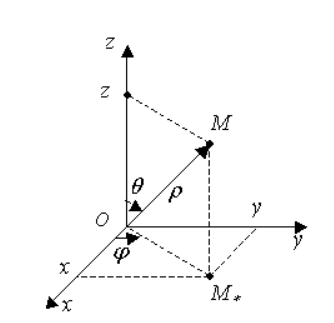
\includegraphics[scale=.600]{coords.png}
\end{figure}

$$\vec \nabla \varphi = \frac{\partial \varphi}{\partial r}\vec e_r$$

$$\vec \nabla \vec \varphi = \frac1{r^2}\frac{\partial}{\partial r}(r^2\varphi(r))$$


\end{document}



















